\chapter{Estrangulamiento del Canal}
\section{Simulación}
\subsection{Simulación (JFET)}

\begin{figure}[H]
    \centering

    \begin{minipage}{0.49\textwidth}
        \centering
        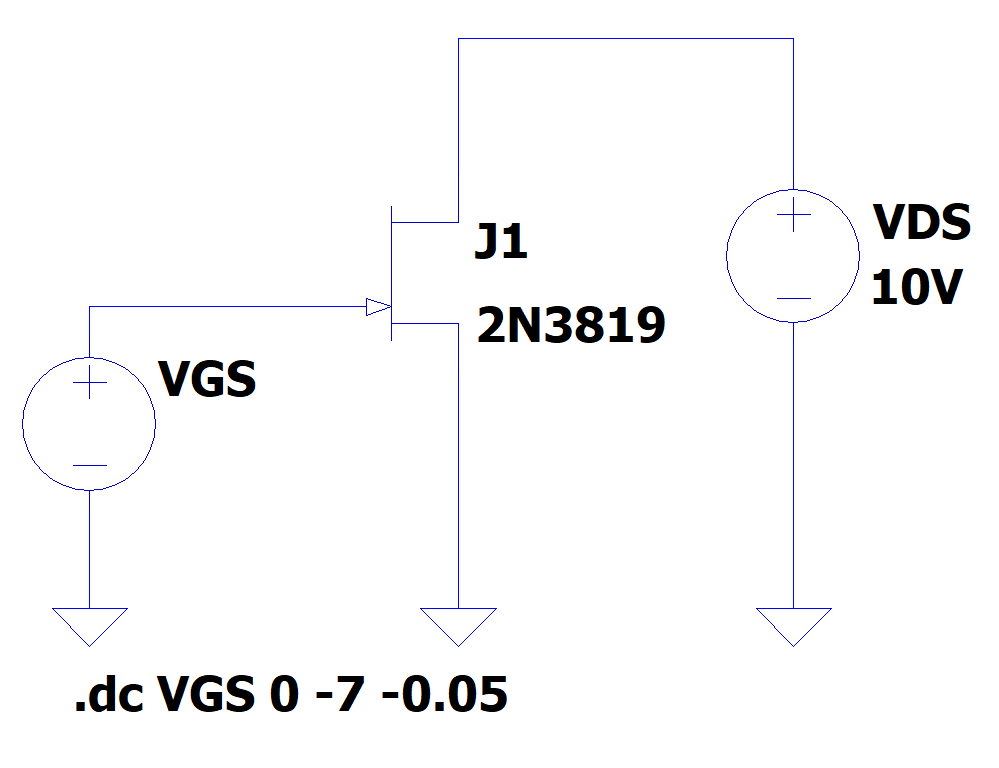
\includegraphics[width=\textwidth]{img/circuito_2N3819_2.png}
        \caption{Primera imagen}
    \end{minipage}
    \hfill
    \begin{minipage}{0.49\textwidth}
        \centering
        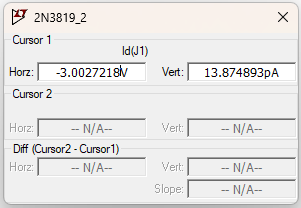
\includegraphics[width=\textwidth]{img/medicion_2N3819_2.png}
        \caption{Segunda imagen}
    \end{minipage}

\end{figure}



\begin{figure}[H]
\centering
\begin{tikzpicture}
\begin{axis}[
    width=16cm,
    height=9cm,
    ymin=-0.05,
    xmax=0,
    xmin=-7,
    xlabel={$V_{GS}$ [V]},
    ylabel={$I_d$ [mA]},
    grid=major,
    minor tick num=1,
    grid=both,
]

\addplot[
    ultra thick,
    blue 
]
table[
    col sep=tab,
    header=true,
    x index=0,
    y index=1,
    y expr=\thisrowno{1}*1000
] {dataTex/2N3819_2.txt};
\addplot[
    only marks,
    mark=*,
    mark size=2.5pt
] coordinates {
    (-3,0)
}
node[
    above left
] {$V_{P}\approx-3\,\mathrm{V}$};

\end{axis}
\end{tikzpicture}
\caption{Curva del diodo 1N4007 en directa, obtenida por simulación}
\end{figure}


\subsection{Simulación (MOSFET)}


\begin{figure}[H]
    \centering

    \begin{minipage}{0.49\textwidth}
        \centering
        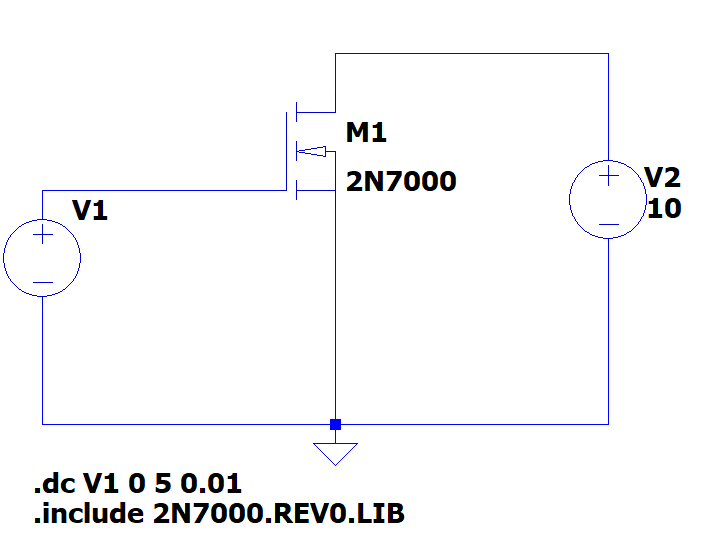
\includegraphics[width=\textwidth]{img/circuito_2N7000_2.png}
        \caption{Primera imagen}
    \end{minipage}
    \hfill
    \begin{minipage}{0.49\textwidth}
        \centering
        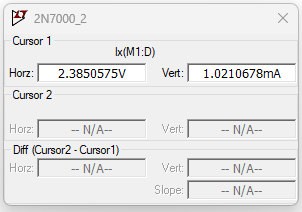
\includegraphics[width=\textwidth]{img/medicion_2N7000_2.png}
        \caption{Segunda imagen}
    \end{minipage}

\end{figure}



\begin{figure}[H]
\centering
\begin{tikzpicture}
\begin{axis}[
    width=16cm,
    height=9cm,
    ymin=-0.05,
    xmax=5,
    xmin=0,
    xlabel={$V_{GS}$ [V]},
    ylabel={$I_d$ [mA]},
    grid=major,
    minor tick num=1,
    grid=both,
]

\addplot[
    ultra thick,
    blue 
]
table[
    col sep=tab,
    header=true,
    x index=0,
    y index=1,
    y expr=\thisrowno{1}*1000
] {dataTex/2N7000_2.txt};
\addplot[
    only marks,
    mark=*,
    mark size=2.5pt
] coordinates {
    (2.384,1)
}
node[
    above left
] {$V_{GS(th)}\approx2.4\,\mathrm{V}$};

\end{axis}
\end{tikzpicture}
\caption{Curva del diodo 1N4007 en directa, obtenida por simulación}
\end{figure}





\section{Implementación en Laboratorio}

\begin{table}[H]
\centering
\caption{Valores registrados para la obtención de $V_{GS(th)}$ fijando $V_{DS}=10$ V nominales.}
\label{tab:valores_vgsth}

\begin{tabular}{|c|c|c|c|}
\hline
$V_{GS}$ Medido [V] & $I_D$ Registrada [mA] &
$V_{GS}$ Medido [V] & $I_D$ Registrada [mA] \\ \hline

0,0 & 0,00 & 2,4 & 0,85 \\ \hline
1,0 & 0,00 & 2,6 & 2,10 \\ \hline
1,5 & 0,01 & 2,8 & 4,20 \\ \hline
1,8 & 0,03 & 3,0 & 6,80 \\ \hline
2,0 & 0,08 & 3,5 & 18,50 \\ \hline
2,2 & 0,25 & 4,5 & 65,00 \\ \hline

\end{tabular}
\end{table}


\begin{figure}[H]
    \centering
    
    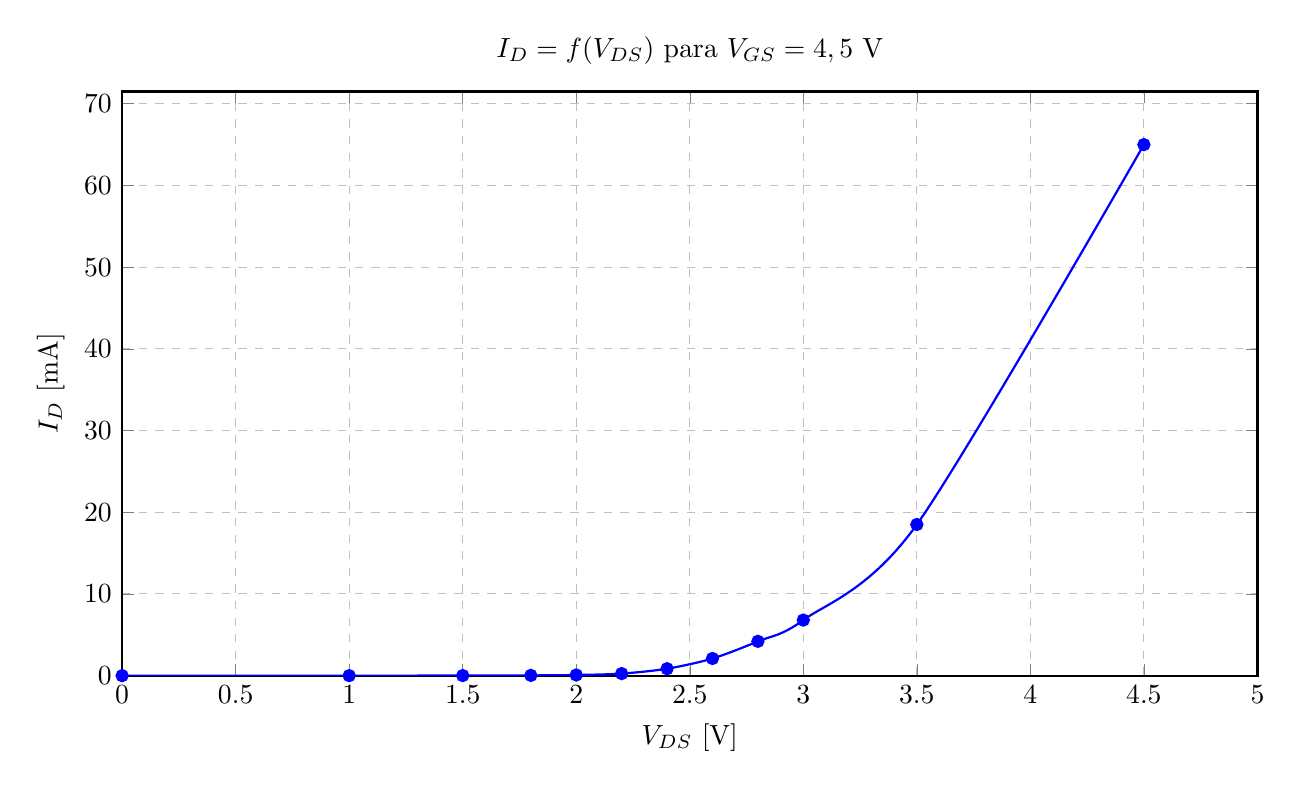
\begin{tikzpicture}
        \begin{axis}[
            width=16cm,
            height=9cm,
            xlabel={$V_{DS}$ [V]},
            ylabel={$I_D$ [mA]},
            title={$I_D=f(V_{DS})$ para $V_{GS}=4,5$ V},
            xmin=0, xmax=5,
            ymin=0,
            grid=both,
            minor grid style={dotted},
            major grid style={dashed},
            thick,
            mark size=2pt,
        ]
        
        \addplot[
            mark=*,
            smooth,
            thick,
            blue
        ] coordinates {
            (0,0)
            (1,0)
            (1.5,0.01)
            (1.8,0.03)
            (2,0.08)
            (2.2,0.25)
            (2.4,0.85)
            (2.6,2.10)
            (2.8,4.2)
            (3,6.80)
            (3.5,18.5)
            (4.5,65)
        };
        
        \end{axis}
    \end{tikzpicture}
    
    \caption{Curva experimental $I_D=f(V_{DS})$ para $V_{GS}=4,5$ V.}
    \label{fig:id_vds}
\end{figure}



